\documentclass[aspectratio=169,xcolor=dvipsnames,UTF8]{beamer}
\usetheme{SimplePlus}

\usepackage{ctex}
\usepackage{CJK}
\usepackage{fontspec}
\usepackage{listings}
\usepackage{listings-ext}
\usepackage{color}
\usepackage{hyperref}
\usepackage{subfigure}
\usepackage{graphicx} % Allows including images
\usepackage{booktabs} % Allows the use of \toprule, \midrule and \bottomrule in tables
\usepackage{caption}
\usepackage{indentfirst}

% -- 压制警告
\PassOptionsToPackage{quiet}{xeCJK}

%图目录配置
\graphicspath{{images/}}
%图注解配置
%\captionsetup{font={tiny}}

\lstset{
	backgroundcolor=gray,
	basicstyle=\small\ttfamily,
	columns=fixed,
	numbers=left,                                           % 在左侧显示行号 
	frame=single,
	framexleftmargin=1pt,
	numbersep=5pt,                                          % 不显示背景边框
	backgroundcolor=\color[RGB]{245,245,244},               % 设定背景颜色
	keywordstyle=\color[RGB]{40,40,255}\bfseries\underbar,  % 设定关键字颜色
	numberstyle=\tiny\footnotesize\color{darkgray},         % 设定行号格式     
	commentstyle=\ttfamily,                                 % 设置代码注释的格式
	stringstyle=\ttfamily\color[RGB]{128,0,0},              % 设置字符串格式
	showstringspaces=false,                                 % 不显示字符串中的空格
	language=bash,                                          % 设置语言
	breaklines = true,
}

% 配置参考文献
\usepackage[hyperref=true,backend=biber,sorting=none]{biblatex}
\addbibresource{reference.bib} %BibTeX数据文件及位置
\setbeamerfont{footnote}{size=\tiny} %调整注脚的文字大小
%\setbeamertemplate{bibliography item}[text]

%----------------------------------------------------------------------------------------
%	标题页
%----------------------------------------------------------------------------------------

% 标题
\title[Web常见问题指北]{Web常见问题指北} 
\subtitle{浏览器同源策略及常见云产品涉及跨域问题和解决方法}

\author[Wei-Zhao] {Wei-Zhao}

\institute[Anchnet] 
{
	Anchen.Net
}
% 按编译日期计
\date{\today}


\begin{document}
	
	%----------------------------------------------------------------------------------------
	% 标题页
	%----------------------------------------------------------------------------------------
	\begin{frame}
		\titlepage
	\end{frame}
	%----------------------------------------------------------------------------------------
	
	
	%----------------------------------------------------------------------------------------
	% 目录页
	%----------------------------------------------------------------------------------------
	\begin{frame}{目录}
		\tableofcontents
	\end{frame}
	%----------------------------------------------------------------------------------------
	
	%同源策略 是由NetScape提出的一个著名的安全策略。所谓的同源,指的是协议,域名,端口相同。浏览器处于安全方面的考虑,只允许本域名下的接口交互,不同源的客户端脚本,在没有明确授权的情况下,不能读写对方的资源。
	%设想这样一种情况:A网站是一家银行,用户登录以后,又去浏览其他的网站,如果其他网站可以读取A网站的Cookie,会发生什么?很显然,如果Cookie包含隐私(比如存款总额),这些信息就会泄漏。更可怕的是Cookie往往用来保存用于的登录状态,如果用户没有退出登录,其他网站就可以冒充用户为所欲为,因为浏览器同时还规定,提交表单不受同源策略的限制。
	%由此可见,同源策略是必须的。如果非同源,那么在请求数据时,浏览器会在控制台中报一个异常,提示拒绝访问。
	
	%------------------------------------------------
	\section{引言}
	%------------------------------------------------
	\begin{frame}{引言-跨域报错}
		\begin{figure}
			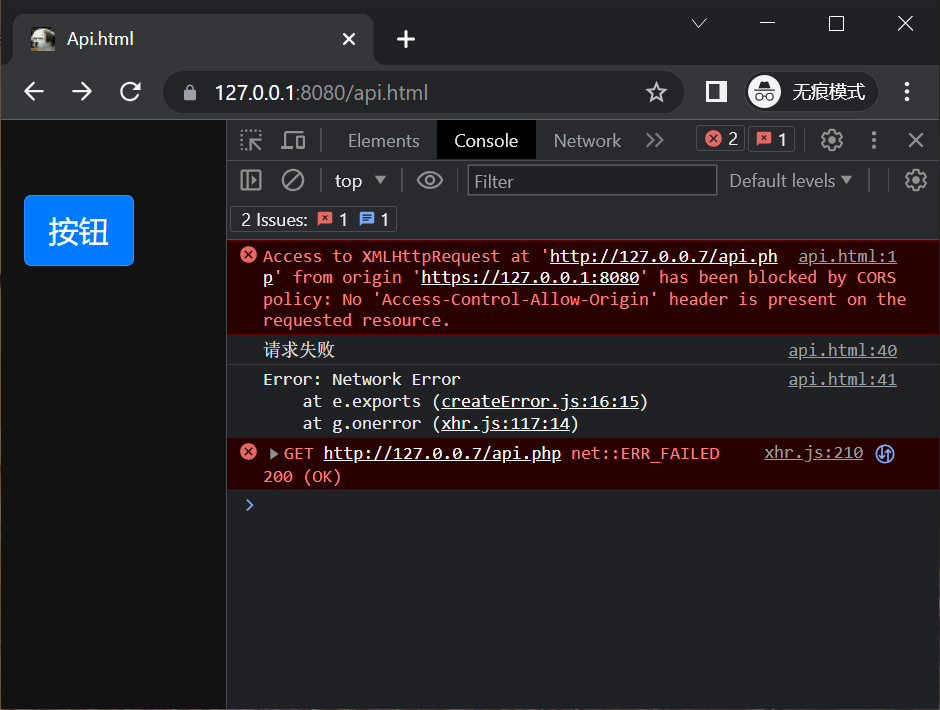
\includegraphics[width=0.48\linewidth]{cors-console-error.png.eps}
			%\caption{ \fontsize{0.5pt}{0pt} 1.1 Chrome控制台错误}
			%\begin{center}
			%	 1.1 Chrome控制台错误
			%\end{center}
			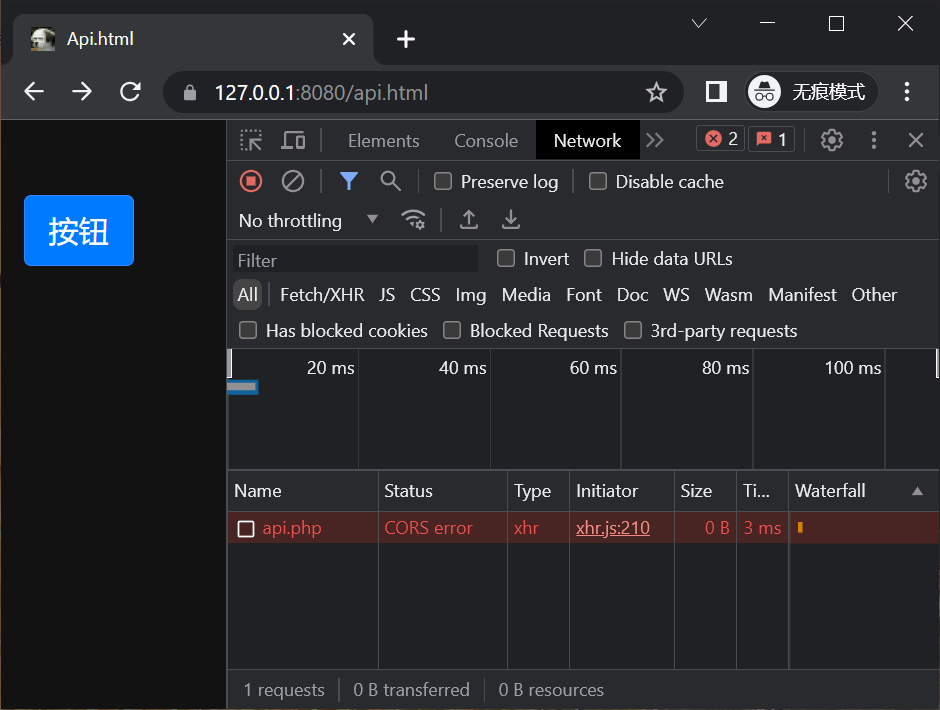
\includegraphics[width=0.48\linewidth]{cors-network-error.png.eps}
			%\caption{ \fontsize{0.5pt}{0pt} 1.2 Chrome控制台网络}
			%\begin{center}
			%	 1.2 Chrome控制台网络
			%\end{center}
		\end{figure}
		%{\songti 宋体}	
		%{\heiti 黑体}
		%{\fangsong 仿宋}
		%{\kaishu 楷书}
	\end{frame}
	
	%------------------------------------------------
	\section{同源策略}
	%------------------------------------------------
	\begin{frame}{同源策略(Same Origin Policy)}
		\begin{block}{}
			\emph{浏览器的同源策略,限制了来自不同源的“document”或脚本,对当前“document”读取或设置某些属性。} 
		\end{block}
		\vspace{2em}
		\setlength{\parindent}{2em}同源策略(Same Origin Policy\footfullcite{web-security})是一种约定,它是浏览器最核心也最基本的安全功能,如果缺少了同源策略,则浏览器的正常功能可能都会受到影响。可以说Web是构建在同源策略的基础之上的,浏览器只是针对同源策略的一种实现。\footfullcite{bmaq}
	\end{frame}
	
	\begin{frame}{存在跨域的情况}
		\begin{table}
			\begin{tabular}{l l c l}
				\toprule
				\textbf{当前页面URL}       & \textbf{被请求的URL}       & \textbf{是否跨域}       & \textbf{原因}       \\
				\midrule
				http://test.com/       & http://test.com/api/data       &       否 &       同源               \\
				http://test.com/       & https://test.com/api/data      &       是 &       协议不同(http/https)\\
				http://test.com/       & http://www.baidu.com           &       是 &       主域名不同           \\
				http://test.com/       & http://api.test.com/api/data   &       是 &       子域名不同           \\
				http://test.com:81/    & https://test.com:446/api/data  &       是 &       端口不同    \\
				\bottomrule
			\end{tabular}
			\caption{1-1 不同源明细 \footfullcite{same-origin_policy}} 
		\end{table}
	\end{frame}
	
	%------------------------------------------------
	\section{如何解决跨域报错}
	%------------------------------------------------
	\begin{frame}{如何解决跨域报错}
		\begin{enumerate}
			\item JSONP 
			\item CORS (跨域资源共享)
			\item Reverse Proxy (反向代理)
		\end{enumerate}
	\end{frame}
	
	
	\begin{frame}{JSONP方案-介绍}
		JSONP\footfullcite{jsonp-wiki}的原理是利用不受浏览器同源策略限制的标签来发起请求。不受同源策略的标签有script、img、link(css)。后面两个标签无法回传数据,通常使用script加载js代码来回传数据。
	\end{frame}
	
	\begin{frame}{JSONP方案-交互时序}
		\begin{figure}
			\includegraphics[width=0.95\linewidth]{images/jsonp.eps}
			\caption{1-1 JSONP交互时序}
		\end{figure}
	\end{frame}
	
	\begin{frame}{JSONP方案-优缺点}
		\begin{columns}[c]
			\column{.45\textwidth}
			\textbf{优点}
			\begin{enumerate}
				\item 兼容性高,能支持古老的浏览器
				\item 实现简单即可轻松跨域
				% \item 
			\end{enumerate}
			\column{.45\textwidth}
			\textbf{缺点}
			\begin{enumerate}
				\item 只支持GET请求
				\item 排错难度大,失败的时候不会返回HTTP状态码
				\item 安全性差容易被XXS攻击
			\end{enumerate}
		\end{columns}
	\end{frame}
	
	
	\begin{frame}{CORS (跨域资源共享)-介绍}
		CORS\footfullcite{cors}是一种服务端软件控制的、基于HTTP响应头的机制。它允许服务器标识除自己以外的源(在“同源策略”有介绍过),并控制浏览器来加载这个服务器的资源。当AJAX发起请求后,浏览器会检查服务端的响应头(Access-Control-Allow-Origin)。如果返回的头中不包含当前发起请求的源,浏览器会直接抛出错误。这个错误无法由JavaScript代码捕获,只能在控制台看到报错。
	\end{frame}
	
	\begin{frame}{CORS (跨域资源共享)-交互时序}
		\begin{figure}
			\includegraphics[width=0.95\linewidth]{images/cros.eps}
			\caption{1-2 CORS交互时序}
		\end{figure}
	\end{frame}
	
	\begin{frame}{如何鉴别是否是简单请求}
		\begin{enumerate}
			\item 请求方法只能是GET、POST、HEAD
			\item 请求头限制这几种字段:Accept、Accept-Language、Content-Language、Content-Type、Last-Event-ID 
			\item Content-Type只能取:application/x-www-form-urlencoded、multipart/form-data、text/plain
		\end{enumerate}
	\end{frame}
	
	\begin{frame}{CORS (跨域资源共享)-优缺点}
		\begin{enumerate}
			\item 需要改造业务代码
			\item 配置项多,比较复杂
			\item 使用当JSON是多一次请求
		\end{enumerate}
	\end{frame}
	
	\begin{frame}{ Reverse Proxy (反向代理)-介绍}
		反向其实还是走的上面的CORS的策略,只不过加了一个中间层。将这边部分请求头改造到Nginx等反向代理服务端上进行处理。
	\end{frame}
	
	\begin{frame}[fragile]{ Reverse Proxy (反向代理)-配置}
		\framesubtitle{The proof uses \textit{reductio ad absurdum}.}
		\begin{lstlisting}
location /api/ {
	add_header Access-Control-Allow-Origin '*' always;
	add_header Access-Control-Allow-Headers '*';
	add_header Access-Control-Allow-Methods '*';
	add_header Access-Control-Allow-Credentials 'true';
	if ($request_method = 'OPTIONS') {
		return 204;
	}
	proxy_set_header Host $http_host;
	proxy_set_header X-Real-IP $remote_addr;
	proxy_set_header X-Forwarded-For $proxy_add_x_forwarded_for;
	proxy_pass http://192.168.1.1:8081/;
}			
		\end{lstlisting}
	\end{frame}
	%-----------------
	\section{总结回顾}
	%-----------------
	\begin{frame}{存在跨域的情况}
		\begin{table}
			\begin{tabular}{l l }
				\toprule
				\textbf{当前页面URL}       & \textbf{被请求的URL}        \\
				\midrule
				https://example.com/index.html &  http://vod.example.com/1.mp4     \\
				https://example.com/index.html &  http://example.com/1.mp4         \\
				\bottomrule
			\end{tabular}
			\caption{1-2 辨析}
		\end{table}
	\end{frame}
	
	%----------------------------------------------------------------------------------------
	% 参考文献页
	%----------------------------------------------------------------------------------------
	\begin{frame}{References}
		%    \footnotesize{
			%        \begin{thebibliography}{99}
				%        	\bibitem{article1}陈立辉,苏伟,蔡川,陈晓云.\emph{基于LaTeX的Web数学公式提取方法研究}[J], 计算机科学,2014(06)
				%        \end{thebibliography}
			%    }
		\printbibliography
	\end{frame}
	
	%----------------------------------------------------------------------------------------
	% 结束页
	%----------------------------------------------------------------------------------------
	
	\begin{frame}
		\Huge{\centerline{\textbf{谢谢观看}}}
	\end{frame}
	
	%----------------------------------------------------------------------------------------
\end{document}